\documentclass[12pt]{article}
\usepackage[utf8]{inputenc}
\usepackage{authblk}
\usepackage{graphicx} % Lib de importar e tratar imagem
\usepackage[portuguese,brazil]{babel} % Manter dois idiomas
\usepackage{fancyhdr} % Configuracao das paginas
\usepackage{float}
\usepackage{xcolor}
\usepackage{titlesec}
\usepackage{background} % Componente de Watermark
\usepackage{hyperref} % utilização de hiperlink em um documento

%Funcao para diminuir tamanho da fonte
\newcommand{\changefont}{%
    \fontsize{9}{12}\selectfont
}

%Document Layout Config
\pagestyle{fancy}
\setlength\headheight{26pt}
\setlength\parindent{0pt}
\fancyhf{}
% Header  Config
\fancyhead[RO]{Estudo da tecnologia SecComp}
\fancyhead[LO]{\includegraphics[width=0.7cm]{Logo.png}}
% Footer  Config
\renewcommand{\footrulewidth}{0.4pt} % Inserir linha no final da pagina "pre-footer"
\fancyfoot[RO]{\includegraphics[width=0.7cm]{Logo.png}}

%Document Specification
\title{Estudo da tecnologia SecComp}
\author{senhasegura}
\affil{Departamento de Segurança e Inovação - SEGi9}
\date{\selectlanguage{portuguese}\today}
\graphicspath{ {img/} }

%Page1 - Capa
\begin{document}
\NoBgThispage % Ignorar background na capa
\maketitle
\begin{center}
\includegraphics{Logo.png}
\end{center}
\begin{center}
\textbf{\LARGE \\CONFIDENCIAL}
\end{center}
\pagenumbering{gobble} % Não contar como página a capa
\pagebreak

% Background a partir da segunda pagina
\backgroundsetup{contents=
\includegraphics{logo.png}, scale=1.5, opacity=0.15, angle=0} % marca d'agua

%Page2 - Executive summary
\section*{\centering{Resumo executivo}}
\vspace*{\fill}
\large{O objetivo deste texto é o de documentar o estudo realizado sobre a tecnologia SecComp e o que essa tecnologia pode ser utilizada para melhorar a segurança do software senhasegura, ferrametna essa desenvolvida pela empresa MT4.}
\vspace*{\fill}
\fancyfoot[CO]{senhasegura\\ \changefont Qualquer reprodução ou distribuição é estritamente proibida sem a aprovação prévia por escrito da empresa MT4.}
\pagebreak

%Indice/Sumario
\tableofcontents
\pagebreak

%Page3
\fancyfoot[CO]{\thepage\\\changefont Qualquer reprodução ou distribuição é estritamente proibida sem a aprovação prévia por escrito da empresa MT4.}
\pagenumbering{arabic}

\section{Introdução}

Um grande número de chamadas do sistema é exposto a todos os processos do usuário, com muitas delas não sendo utilizadas durante toda a vida útil do processo. À medida que as chamadas do sistema mudam, os bugs são encontrados e erradicados. Um certo subconjunto de aplicativos de userland se beneficia por ter um conjunto reduzido de chamadas de sistema disponíveis. O conjunto resultante reduz a superfície total do  kernel exposta ao aplicativo. A filtragem de chamadas do sistema destina-se ao uso com esses aplicativos.\\

A filtragem Seccomp fornece um meio para um processo especificar um filtro para chamadas de sistema recebidas. O filtro é expresso como um programa Berkeley Packet Filter (BPF), como acontece com os filtros de socket. Isso permite a filtragem expressiva de chamadas do sistema usando uma linguagem de programa de filtro com um longo histórico de exposição à área de usuário e um conjunto de dados direto.

\section{Chamada de Sistema/SysCall}

Quando falamos sobre os Sistemas Operacionais sob o ponto de vista da programação, citamos que uma de suas funções é fornecer algumas abstrações, de modo que o usuário não tenha que se preocupar com coisas específicas e complexas, além de gerenciar recursos de hardware (como memória e processamento).\\

As chamadas de sistemas são funções (interfaces) usadas pelos aplicativos para solicitar a execução de algum serviço ao kernel do sistema operacional. Por isso, as chamadas de sistemas são instruções com maior privilégio quando comparadas às outras instruções.\\

Com as chamadas de sistemas é possível, por exemplo, definir acesso a recursos de baixo nível como alocação de memória, periféricos e arquivos. Além disso, são as chamadas de sistemas que permitem a criação e a finalização de processos.\\

O programador normalmente não utiliza as chamadas de sistema no seu código. Ele utiliza uma função de biblioteca que é transformada em uma ou mais chamadas de sistema quando o código executável é gerado e há necessidade de pedir um serviço ao kernel.\\

\begin{figure}[H]
	\centering
	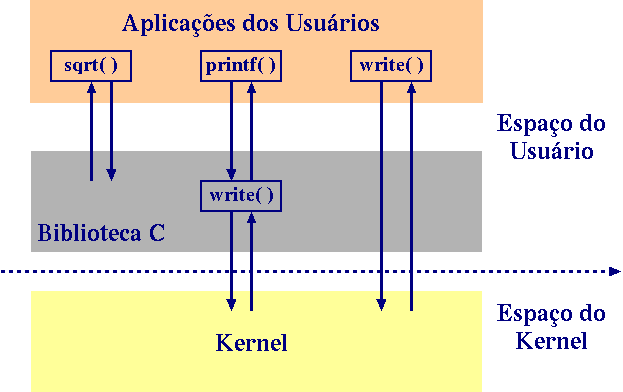
\includegraphics[scale=0.63]{img/syscall.png}
	\caption{Funcionamento da chamada de sistema do Sistema Operacional}
\end{figure}

O programador pode usar as chamadas de sistema no seu código se, por exemplo, está usando a Linguagem C. Com isto, ele ganha rapidez na compilação do programa (não precisa fazer a conversão), mas diminui a portabilidade do código (o formato das chamadas pode variar com as arquiteturas).\\

Em todo projeto de sistema operacional os projetistas sempre se preocuparam em garantir a integridade do próprio sistema operacional, protegendo o núcleo e o serviços do sistema operação de acessos indevidos por uma aplicação do usuário. Caso uma aplicação do usuário tenha acesso ao núcleo e realize alguma operação que altere sua integridade então todo o sistema ficará comprometido. Muitos sistemas operacionais utilizam um mecanismo de segurança implementado no hardware do processador e conhecido como modo de acesso.\\

Este mecanismo de proteção funciona através do conceito de modo usuário(userspace) ou modo kernel(kernel space).\\

\textbf{“User Space}\\

Quando o processador trabalha em  modo usuário, uma aplicação tem acesso a apenas algumas instruções não-privilegiadas,tendo acesso a um número reduzido de instruções\\

\textbf{“Kernel Space”}\\

Quando o processador está em modo kernel a aplicação sendo executada tem acesso a todo o conjunto de instruções do processador, tem acesso as instruções privilegiadas.\\

\subsection{GNU/Linux}

Como obter informações sobre as chamadas de sistemas utilizadas por um determinado comando do gnu/linux. No exemplo abaixo, é exemplificado como obter informações sobre o comando chown.

\begin{table}[H]
	\begin{tabular}{|l|}
	\hline
	\$ man -k chown\\
	(...)\\
	chown (2)            - change ownership of a file\\
	(...)\\
	\$ man 2 chown\\
	\hline
	\end{tabular}
\end{table}

Utilizando o aplicativo strace para obetr mais informações sobre quais chamadas de sistemas são utilizadas quando um determinado aplicativo é executado. No exemplo abaixo, é executado o comando "echo" que escreve dados, "oi", em um arquivo.

\begin{table}[H]
	\begin{tabular}{|l|}
	\hline
	\$ strace echo "oi"  \textgreater\ src/oi.txt\\
	(...)\\
	write(1, "oi", 3)\\
	close(1)\\
	close(2)\\
	exit\_group(0)\\
	\hline
	\end{tabular}
\end{table}

\section{SecComp}

Seccomp (abreviação de Secure Computing Mode) é um recurso de segurança de computador que fornece um mecanismo de sandboxing de aplicativos no kernel do Linux. Com o Iptables, é possivel filtrar endereços IP, já com o seccomp, é possivel filtrar chamadas de sistema, syscall.\\

Na primeira versão do Seccomp, ano de 2005 e a versão do kernel do Linux era a versão 2.6.12, é permite que um processo faça uma transição unidirecional para um estado "seguro" onde não pode fazer nenhuma chamada de sistema, exceto exit(), sigreturn(), read() e write em arquivo já abertos. Caso tente qualquer outra chamada de sistema, o kernel encerrará o processo com SIGKILL ou SIGSYS.\\

Em 2012, kernel Linux 3.5, o "seccomp mode 2" (ou "seccomp filter mode") foi adicionado ao Linux. Foi adicionado um segundo modo para o seccomp: SECCOMP\_MODE\_FILTER. Utilizando este modo, é possivel fazer com que os processos possam especificar quais chamadas de sistema são permitidas. Ao usar um miniprograma na linguagem Berkeley Packet Filter (BPF), os processos podem restringir as chamadas do sistema inteiramente ou apenas para determinados valores de argumento.\\

\subsection{SecComp e Docker}

O Secure Computing Mode (seccomp) é um recurso do kernel que permite filtrar chamadas do sistema para o kernel a partir de um container. A combinação de chamadas "restritas" e "permitidas" são organizadas em perfis, e pode-se passar diferentes perfis para diferentes containers. O Seccomp fornece controle mais refinado do que recursos, dando ao atacante um número limitado de syscalls do container.\\

Como verificar se o kernel suporta seccomp.\\

\begin{table}[H]
	\begin{tabular}{|l|}
	\hline
	\$ grep SECCOMP /boot/config-\$(uname -r)\\ 
    CONFIG\_HAVE\_ARCH\_SECCOMP=y\\
    CONFIG\_HAVE\_ARCH\_SECCOMP\_FILTER=y\\
    CONFIG\_SECCOMP=y\\
    CONFIG\_SECCOMP\_FILTER=y\\
	\hline
	\end{tabular}
\end{table}

A opção docker que é usada para operar com seccomp é --security-opt. Para usar explicitamente uma política para um  contêiner, o comando será:

\begin{table}[H]
	\begin{tabular}{|l|}
	\hline
	\$ docker run $--$security$-$opt seccomp=\textless profile\textgreater.json \textless container\textgreater\\
	\hline
	\end{tabular}
\end{table}

Neste modo de execução, o seccomp trabalha em modo não-confinado.

\begin{table}[H]
	\begin{tabular}{|l|}
	\hline
	\$ docker run -it $--$security$-$opt seccomp=unconfined alpine\\
	\hline
	\end{tabular}
\end{table}

Alguns exemplos de arquivos de configuração do seccomp para container.\\
\url{https://raw.githubusercontent.com/docker/labs/master/security/seccomp/seccomp-profiles/default.json}

\subsection{Exemplo}

No exemplo abaixo, será liberado a execução de todos os aplicativos, \textbf{SCMP\_ACT\_ALLOW}, exceto os aplicativos mkdir, chmod e chown, \textbf{SCMP\_ACT\_ERRNO}.

\begin{figure}[H]
	\centering
	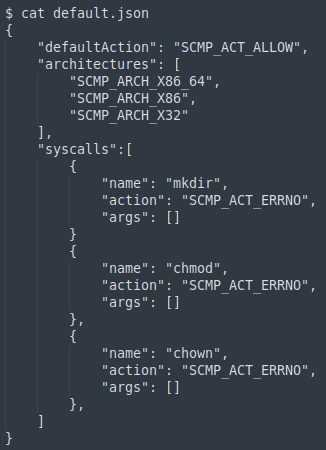
\includegraphics[scale=0.63]{img/default.png}
	\caption{Exemplo de uma política do SecComp}
\end{figure}

Testando a configuração do seccomp que impede a criação de diretórios dentro do container.\\

\begin{table}[H]
	\begin{tabular}{|l|}
	\hline
	\$ docker run $-$it $--$security-opt seccomp=block\_mkdir.json alpine bash\\
	\# mkdir teste\\
	mkdir: cannot create directory 'teste': Operation not permitted\\
	\hline
	\end{tabular}
\end{table}

\section{SecComp x Apparmor}

\textbf{Seccomp} é um recurso do kernel do Linux que permite que um programa que é executado no Espaço do Usuário configure filtros para as chamadas de sistema, syscall. Esses filtros especificam quais chamadas de sistema são permitidas e quais argumentos elas podem ter. É um filtro de nível muito baixo e que reduz a área de superfície de ataque do kernel Linux. Por exemplo, um bug em keyctl() que permite chamadas simples para essa syscall para elevar privilégios não seria necessariamente utilizada para privesc em um programa que tenha acesso restrito a essa chamada.\\

\textbf{AppArmor} é uma estrutura de controle de acesso obrigatório que funciona como um LSM (Linux Security Module). Ele é usado para colocar em uma lista de itens permitidos ou bloqueados o acesso de um programa ou um objeto (arquivo, caminho, etc.). O AppArmor pode ser usado para permitir que um programa tenha acesso de leitura ao /etc/passwd, mas não ao /etc/shadow. As políticas também podem ser usadas para restringir recursos ou até mesmo limitar o acesso à rede.\\

Resumindo,
\begin{itemize}
	\item O Secomp reduz a chance de uma vulnerabilidade do kernel ser explorada com sucesso;
	\item O AppArmor impede que um aplicativo acesse arquivos que ele não deveria acessar;
\end{itemize}

\pagebreak
%Copyright
\vspace*{\fill}
\begin{flushright}
	\underline{\textit{Copyright}}\\
	All rights reserved to MT4 Tecnologia LTDA.\bigskip

	\underline{\textit{Documment Control}}\\
	Caio Abreu Ferreira - SEGi9\bigskip

	\underline{\textit{Contact}}\\
	Support [support@senhasegura.com]\bigskip
\end{flushright}

\pagebreak

\end{document}